\section*{Results}

\subsection*{Conditional transport between vibrational modalities}

\mname\ learns a velocity field conditioned on the source spectrum, current spectral state, flow time and target modality (Fig.~\ref{fig:pipeline}). Spectra are normalized sample-wise and represented as ordered one-dimensional sequences. A patch embedding groups neighbouring wavenumber bins, fixed sinusoidal positions encode their order, and eight SpectraDiT blocks exchange information across the sequence. Time, modality and global source features condition the blocks through adaptive layer normalization. Separate checkpoints implement IR$\rightarrow$Raman and Raman$\rightarrow$IR translation.

Training matches the velocity along an interpolation between paired source and target spectra. Peak-weighted reconstruction, derivative matching and local optimal transport provide additional endpoint supervision. At inference, eight Euler steps evolve the source into a normalized target prediction. Output projection enforces the interval $[0,1]$. Intermediate states expose the numerical transformation without implying a physical trajectory.

\subsection*{Translation accuracy and transfer across chemical domains}

\begin{figure}[htbp]
    \centering
    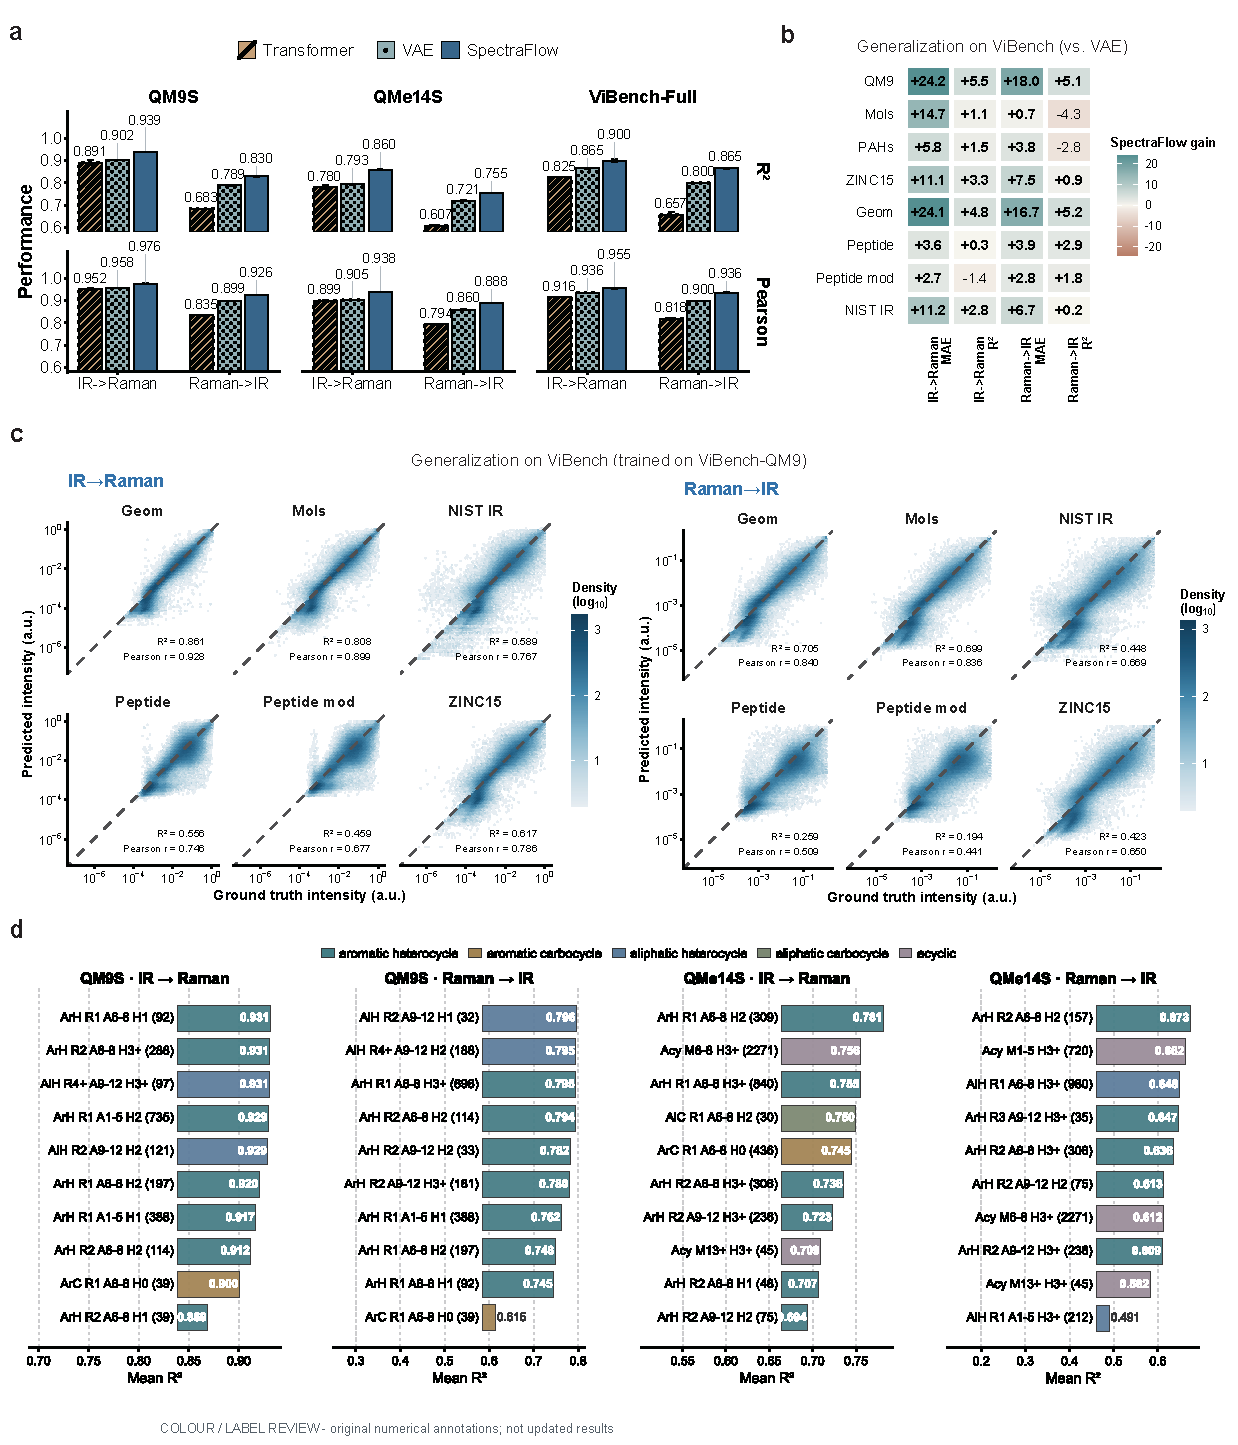
\includegraphics[width=\linewidth]{figs/results/result_1_draw_arial.pdf}
    \caption{\textbf{In-distribution performance and cross-dataset generalization of \mname.}
\textbf{a,} Translation performance of the Transformer, VAE, and \mname\ on QM9S, QMe14S, and ViBench-Full in both directions.
\textbf{b,} Cross-dataset gains of \mname\ over VAE across eight ViBench domains after training on ViBench-QM9, reported as MAE reduction and $R^2$ improvement.
\textbf{c,} Predicted versus ground-truth intensity distributions on six held-out ViBench domains without per-dataset tuning.
\textbf{d,} In-distribution $R^2$ stratified by Murcko scaffold class for QM9S and QMe14S; classes contain at least 30 test molecules.}
    \label{fig:quantitative_result}
\end{figure}

\begin{table}[!htb]
\centering
\caption{\textbf{Bidirectional translation on QM9S, QMe14S and ViBench-Full.}
Values are mean $\pm$ s.d. over four model-initialization seeds on fixed test partitions. VAE and Transformer denote the reconstruction baselines specified in Methods; \mname\ uses conditional flow matching with a one-dimensional SpectraDiT backbone. Bold denotes the best mean. Asterisks denote adjusted $p<0.05$ in two-sided paired Wilcoxon tests against the strongest baseline, with Holm--Bonferroni correction as described in Methods.
Predictions are rescaled using the paired target's minimum and maximum for evaluation on the dataset's native intensity scale. RMSE magnitudes are therefore not comparable across datasets; the large QMe14S Raman values reflect its intensity scale. This reporting convention requires target statistics and does not demonstrate prediction of unknown absolute intensities. Per-spectrum $R^2$ and Pearson $r$ are invariant to the shared affine rescaling.
}
\label{tab:reconstruction}
\scriptsize
\setlength{\tabcolsep}{3.6pt}
\renewcommand{\arraystretch}{1.15}
\begin{tabular}{llcccc}
\toprule
Task & Model & R$^2 \uparrow$ & Pearson $\uparrow$ & RMSE $\downarrow$ & SSIM $\uparrow$ \\
\midrule
\multicolumn{6}{l}{\bfseries\itshape  QM9S\ (\# test: 19,474)} \\
\midrule
\multirow{3}{*}{IR $\rightarrow$ Raman}
& VAE       & $0.902_{\pm 0.001}$ & $0.958_{\pm 0.000}$ & $6.664_{\pm 0.037}$ & $0.940_{\pm 0.002}$ \\
& Transformer & $0.891_{\pm 0.012}$ & $0.952_{\pm 0.006}$ & $6.921_{\pm 0.355}$ & $0.933_{\pm 0.007}$ \\
& \mname\ & $\mathbf{0.939_{\pm 0.001}}$* & $\mathbf{0.976_{\pm 0.001}}$* & $\mathbf{5.129_{\pm 0.036}}$* & $\mathbf{0.963_{\pm 0.001}}$* \\
\cmidrule(lr){1-6}
\multirow{3}{*}{Raman $\rightarrow$ IR}
& VAE & $0.789_{\pm 0.002}$ & $0.899_{\pm 0.001}$ & $8.222_{\pm 0.036}$ & $0.873_{\pm 0.002}$ \\
& Transformer & $0.683_{\pm 0.002}$ & $0.835_{\pm 0.002}$ & $10.178_{\pm 0.050}$ & $0.783_{\pm 0.002}$ \\
&\mname & $\mathbf{0.830_{\pm 0.003}}$* & $\mathbf{0.926_{\pm 0.001}}$* & $\mathbf{7.007_{\pm 0.044}}$* & $\mathbf{0.908_{\pm 0.001}}$* \\
\midrule
\multicolumn{6}{l}{\bfseries\itshape QMe14S\ (\# test: 27,916)} \\
\midrule
\multirow{3}{*}{IR $\rightarrow$ Raman}
& VAE       & $0.793_{\pm 0.004}$ & $0.905_{\pm 0.000}$ & $8727_{\pm 168.4}$  &$0.879_{\pm 0.002}$  \\
& Transformer & $0.780_{\pm 0.009}$  & $0.899_{\pm 0.005}$  & $8972_{\pm 15.39}$  & $0.868_{\pm 0.005}$  \\
& \mname\ & $\mathbf{0.860_{\pm 0.001}}$*  & $\mathbf{0.938_{\pm 0.000}}$*  & $\mathbf{6949_{\pm 129.6}}$*  & $\mathbf{0.921_{\pm 0.000}}$* \\
\cmidrule(lr){1-6}
\multirow{3}{*}{Raman $\rightarrow$ IR}
& VAE       & $0.721_{\pm 0.002}$ & $0.860_{\pm 0.001}$ & $4.084_{\pm 0.024}$ & $0.823_{\pm 0.001}$ \\
& Transformer & $0.607_{\pm 0.002}$ & $0.794_{\pm 0.002}$ & $4.877_{\pm 0.011}$ & $0.729_{\pm 0.004}$ \\
& \mname & $\mathbf{0.755_{\pm 0.001}}$* & $\mathbf{0.888_{\pm 0.000}}$* & $\mathbf{3.630_{\pm 0.043}}$* & $\mathbf{0.863_{\pm 0.001}}$* \\
\midrule
\multicolumn{6}{l}{\bfseries\itshape ViBench-Full\ (\# test: 13,793)} \\
\midrule
\multirow{3}{*}{IR $\rightarrow$ Raman}
& VAE       & $0.865_{\pm 0.001}$  & $0.936_{\pm 0.000}$  & $0.031_{\pm 0.000}$  & $0.926_{\pm 0.001}$ \\
& Transformer &  $0.825_{\pm 0.000}$  & $0.916_{\pm 0.001}$  & $0.035_{\pm 0.000}$  & $0.902_{\pm 0.001}$ \\
&\mname\  &  $\mathbf{0.900_{\pm 0.006}}$* & $\mathbf{0.955_{\pm 0.003}}$* & $\mathbf{0.022_{\pm 0.001}}$* & $\mathbf{0.948_{\pm 0.003}}$* \\
\cmidrule(lr){1-6}
\multirow{3}{*}{Raman $\rightarrow$ IR}
& VAE       &   $0.800_{\pm 0.000}$  & $0.900_{\pm 0.000}$  & $0.033_{\pm 0.000}$  & $0.887_{\pm 0.002}$\\
& Transformer &  $0.657_{\pm 0.011}$  & $0.818_{\pm 0.005}$  & $0.046_{\pm 0.000}$  & $0.789_{\pm 0.003}$ \\
& \mname\  &  $\mathbf{0.865_{\pm 0.002}}$* & $\mathbf{0.936_{\pm 0.001}}$* & $\mathbf{0.022_{\pm 0.001}}$* & $\mathbf{0.928_{\pm 0.002}}$* \\

\bottomrule
\end{tabular}
\renewcommand{\arraystretch}{1.0}
\end{table}

\mname\ has the highest mean $R^2$, Pearson correlation and SSIM, and the lowest RMSE, among the three models in all six dataset--direction comparisons (Table~\ref{tab:reconstruction}). For IR$\rightarrow$Raman, $R^2$ reaches $0.939$, $0.860$ and $0.900$ on QM9S, QMe14S and ViBench-Full, respectively. Relative to VAE, the strongest baseline by RMSE in each case, these results correspond to approximately $23\%$, $20\%$ and $29\%$ lower RMSE. Raman$\rightarrow$IR follows the same ranking on these benchmarks: $R^2$ increases from $0.789$ to $0.830$ on QM9S, from $0.721$ to $0.755$ on QMe14S, and from $0.800$ to $0.865$ on ViBench-Full.

A one-pass SpectraDiT-Direct comparison provides context for the role of the backbone (Supplementary Table~\ref{tab:direct-ablation}). Direct retains the velocity-network architecture but predicts a residual with one network evaluation. It reaches $R^2=0.910$ for IR$\rightarrow$Raman and $0.806$ for Raman$\rightarrow$IR on QM9S, compared with $0.939$ and $0.830$ for eight-step Flow. Direct therefore retains much of the endpoint accuracy. Its shorter optimization budget and lower endpoint-loss coefficient, however, mean that this comparison does not isolate the effect of integration.

For transfer evaluation, models are trained on the ViBench-QM9 source domain and evaluated on its supplied QM9 test set and seven held-out domains: Mols, PAHs, ZINC15, GEOM, Peptide, Peptide-mod and NIST-IR~\citep{lu2025vib2mol}. No domain-specific fine-tuning or additional split is applied. \mname\ lowers MAE relative to VAE on all eight evaluation sets in both directions (Fig.~\ref{fig:quantitative_result}b; Supplementary Table~\ref{tab:vae-vibraflow-main}). The mean relative reductions across the eight sets are approximately $12.2\%$ for IR$\rightarrow$Raman and $7.5\%$ for Raman$\rightarrow$IR. IR$\rightarrow$Raman reductions approach $24\%$ on QM9 and GEOM.

The transfer advantage depends on the metric. $R^2$ improves on seven of eight sets for IR$\rightarrow$Raman and six of eight for Raman$\rightarrow$IR. It decreases for IR$\rightarrow$Raman on Peptide-mod and for Raman$\rightarrow$IR on Mols and PAHs despite lower MAE. On PAHs, IR$\rightarrow$Raman $R^2$ remains negative for both models. Intensity-density plots illustrate the variation across domains, and scaffold-stratified results show variation within QM9S and QMe14S (Fig.~\ref{fig:quantitative_result}c,d). Scaffold classes describe subgroups of random test partitions; they do not constitute scaffold-disjoint evaluation.

The endpoint-supervision comparison increases the probability of computing the endpoint loss from $0.1$ to $0.5$. In the reported sixteen comparisons, MAE decreases and $R^2$ and Pearson correlation increase, with a median relative MAE reduction of approximately $8.1\%$. Because the loss is reweighted by the inverse sampling probability, its expected coefficient remains fixed. This comparison therefore changes the frequency and stochasticity of endpoint supervision, rather than simply increasing its expected weight.

\subsection*{Experimental inputs and cross-library evaluation}

Two evaluations examine measurement-domain shifts (Fig.~\ref{fig:experimental_validation}). The first applies a QM9S-trained IR$\rightarrow$Raman model directly to experimental NIST IR spectra and compares predictions with computed QM9S Raman targets. Molecular matching yields 84 overlaps: 76 stereochemistry-aware exact matches and eight connectivity-only matches. Median Pearson correlations are $0.42$ and $0.40$, respectively. Selected exact-match examples reach $r=0.673$, $0.671$ and $0.644$, but the full distribution shows substantially lower correspondence than the controlled computed-spectrum benchmarks. This tests a change in the source measurement domain, rather than establishing generalization to previously unseen molecular identities.

The second evaluation trains a separate model on cross-library OpenSpecy/RRUFF pairs and tests it on 147 pairs from held-out RRUFF identifiers. The development pool contains 590 identifiers and the external test contains 147 identifiers spanning 135 mineral names. The median test correlation is $0.31$ for raw spectra and $0.34$ after baseline correction of predictions and references. Selected records labelled rutile, cassiterite and staurolite reach correlations of $0.953$, $0.942$ and $0.852$. These selected cases show what is attainable for some records; they do not represent average test performance. Identifier matching also does not ensure common specimens or acquisition conditions, and 72 test mineral names occur in the development pool under different identifiers.

The NIST error profile localizes the largest mean normalized discrepancies to approximately $2800$--$3200\,\mathrm{cm}^{-1}$ (Fig.~\ref{fig:experimental_validation}e). The shaded $2200$--$2450\,\mathrm{cm}^{-1}$ interval is a reference region; the error profile alone does not establish the cause of any discrepancy. These evaluations quantify incomplete correspondence under measurement shifts and motivate calibration with paired experimental spectra.

\begin{figure}[htbp]
    \centering
    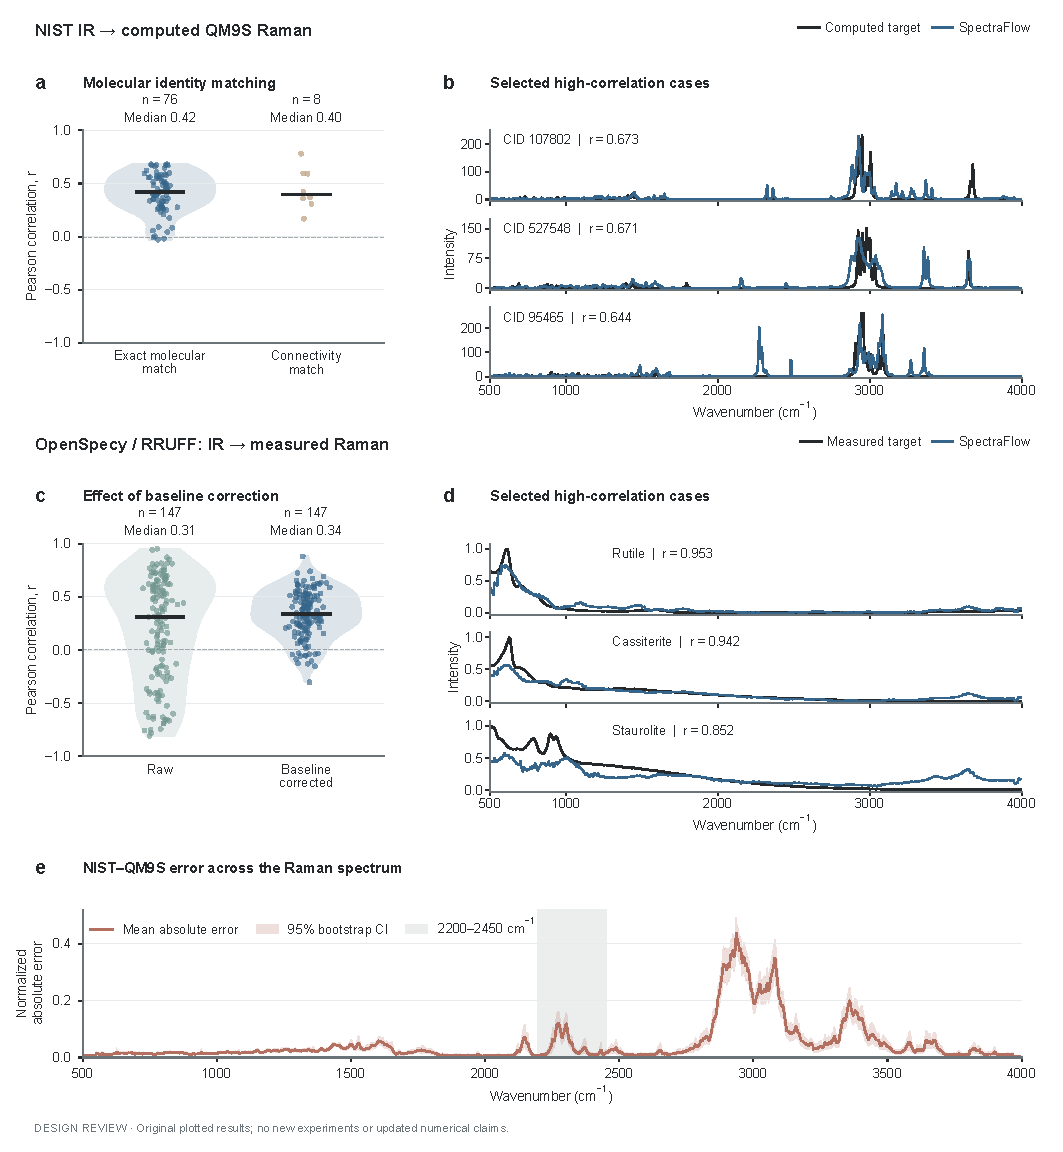
\includegraphics[width=0.98\linewidth]{figs/results/result_4_draw_arial.pdf}
    \caption{\textbf{Experimental-input and cross-library IR$\rightarrow$Raman transfer of \mname.}
\textbf{a,} Pearson correlations for experimental NIST IR inputs against identity-matched computed QM9S Raman targets.
\textbf{b,} Three selected high-correlation NIST--QM9S predictions; targets are computed Raman spectra.
\textbf{c,} Pearson distributions for 147 held-out OpenSpecy/RRUFF pairs before and after baseline correction.
\textbf{d,} Selected high-correlation cross-library predictions against measured Raman targets. The selected cases in b and d do not summarize population-average accuracy.
\textbf{e,} Wavenumber-resolved normalized absolute error across the NIST--QM9S matches; shading denotes the 95\% bootstrap confidence interval. The grey interval marks $2200$--$2450\,\mathrm{cm}^{-1}$ for reference.}
    \label{fig:experimental_validation}
\end{figure}

\subsection*{Peak-resolved errors and intermediate spectral states}

\begin{figure}[htbp]
    \centering
    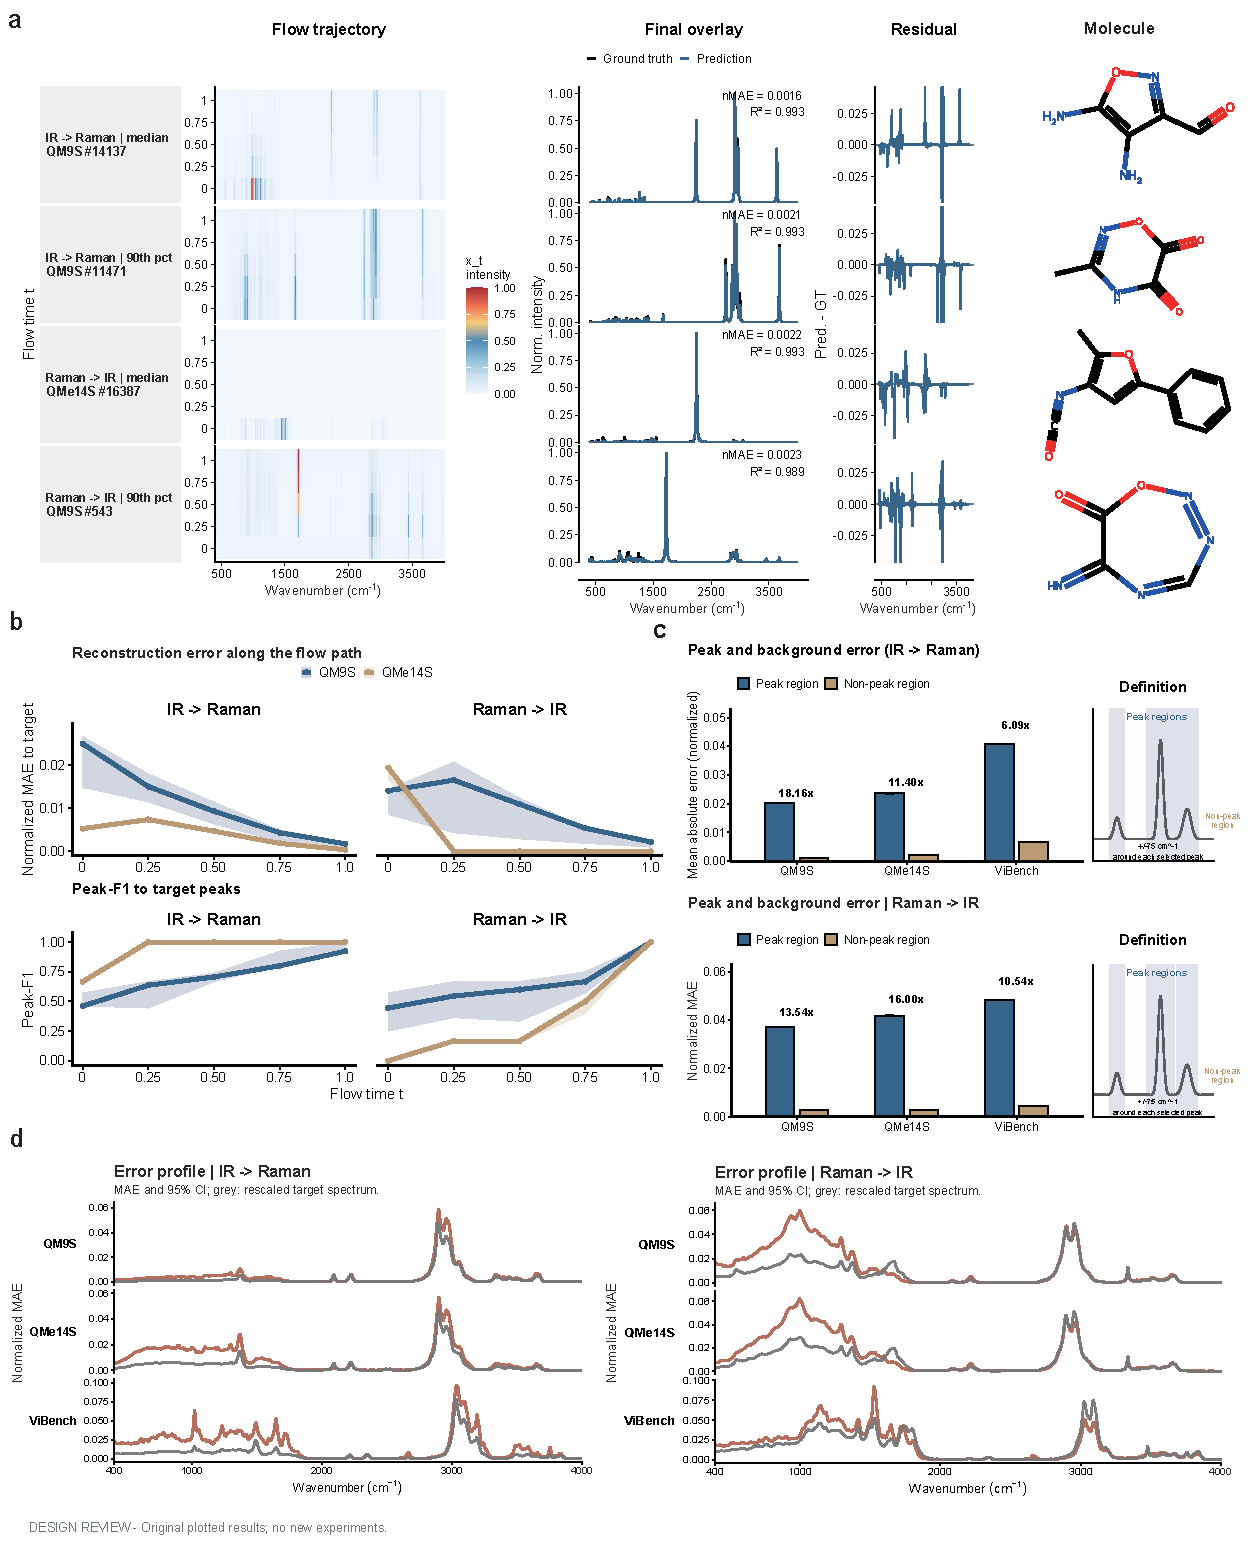
\includegraphics[width=0.97\linewidth]{figs/results/result_2_draw_polished.pdf}
    \caption{\textbf{Learned conversion trajectories and peak-localized prediction error.}
\textbf{a,} Four selected cases: IR$\rightarrow$Raman, QM9S \#14137 and \#11471; Raman$\rightarrow$IR, QMe14S \#16387 and QM9S \#543. Columns show intermediate spectral states, endpoint overlays, residuals and molecular structures. Black curves denote targets and blue curves predictions.
\textbf{b,} Normalized MAE and peak-F1 along the learned flow path. Colour denotes dataset. Flow time describes the model trajectory, not physical molecular dynamics.
\textbf{c,} Peak-region and background errors for both translation directions. Peak regions span $\pm75\,\mathrm{cm}^{-1}$ around selected target peaks; labels give peak/background error ratios.
\textbf{d,} Wavenumber-resolved normalized MAE and 95\% confidence intervals. Grey curves show mean target spectra rescaled for visual comparison.}
    \label{fig:case_study}
\end{figure}

Residual errors are concentrated near spectral peaks (Fig.~\ref{fig:case_study}c,d). Defining peak regions as the union of $\pm75\,\mathrm{cm}^{-1}$ windows around detected target peaks, the peak-to-background normalized error ratios are $18.2$, $11.4$ and $6.1$ for IR$\rightarrow$Raman on QM9S, QMe14S and ViBench, respectively. The corresponding Raman$\rightarrow$IR ratios are $13.5$, $16.0$ and $10.5$. These ratios describe where errors occur; they do not establish their cause.

A separate peak-matching analysis covers all $19{,}474$ QM9S test spectra. At a $20\,\mathrm{cm}^{-1}$ tolerance, IR$\rightarrow$Raman recovers $80.9\%$ of reference peaks, compared with $68.7\%$ for Raman$\rightarrow$IR (Supplementary Fig.~\ref{fig:qm9s_peak_resolved}). High correlations between matched peak intensities coexist with missed peaks, illustrating why aggregate spectral similarity does not fully describe local fidelity.

Selected trajectories show how predictions develop during integration (Fig.~\ref{fig:case_study}a,b). The illustrated endpoints reach approximately $R^2=0.99$ and normalized MAE of $0.0016$--$0.0023$. Along the plotted paths, target MAE generally decreases and peak-F1 increases, although some intermediate steps temporarily increase error. The states are numerical model outputs and need not correspond to realizable molecular spectra. They complement endpoint metrics by exposing where intensity is redistributed during prediction.

\subsection*{Frozen embeddings support molecular-descriptor prediction}

We next test the representations learned during spectral translation (Fig.~\ref{fig:quantitative_result_3}). A model trained on ViBench-QM9 is frozen, and source-generated final-block features at flow time $\tau=0.5$ are mean-pooled. Dataset-specific ridge probes predict ten RDKit descriptors using five shared random train--test splits. The eight evaluation sets include the QM9 source-domain test set and seven held-out domains. Feature comparisons use raw IR, raw Raman, Flow embeddings, Morgan fingerprints and concatenated Flow--fingerprint features. Molecular structures provide descriptor labels and fingerprints; they are not inputs to the spectral translator.

Flow embeddings make the descriptors more accessible to linear prediction than raw spectra in the reported comparisons (Fig.~\ref{fig:quantitative_result_3}b,c). On GEOM, for example, LogP $R^2$ increases from approximately $0.11$ with raw Raman features to approximately $0.70$ with Flow embeddings. UMAP projections illustrate property-associated organization but are not used as evidence of predictive accuracy (Fig.~\ref{fig:quantitative_result_3}a). Because the downstream probes are fitted within each dataset, the evaluation tests transfer of the frozen encoder rather than zero-shot transfer of a property predictor.

Morgan fingerprints remain a strong reference for descriptors calculated from molecular structure. Adding Flow features yields task-dependent changes, including absolute $R^2$ gains approaching $0.15$ and decreases on other property--dataset pairs (Fig.~\ref{fig:quantitative_result_3}d). Changes are expressed as absolute differences in $R^2$. The mixed gains support complementarity for some linear probes, rather than a uniform advantage from concatenation.

\begin{figure}[htbp]
    \centering
    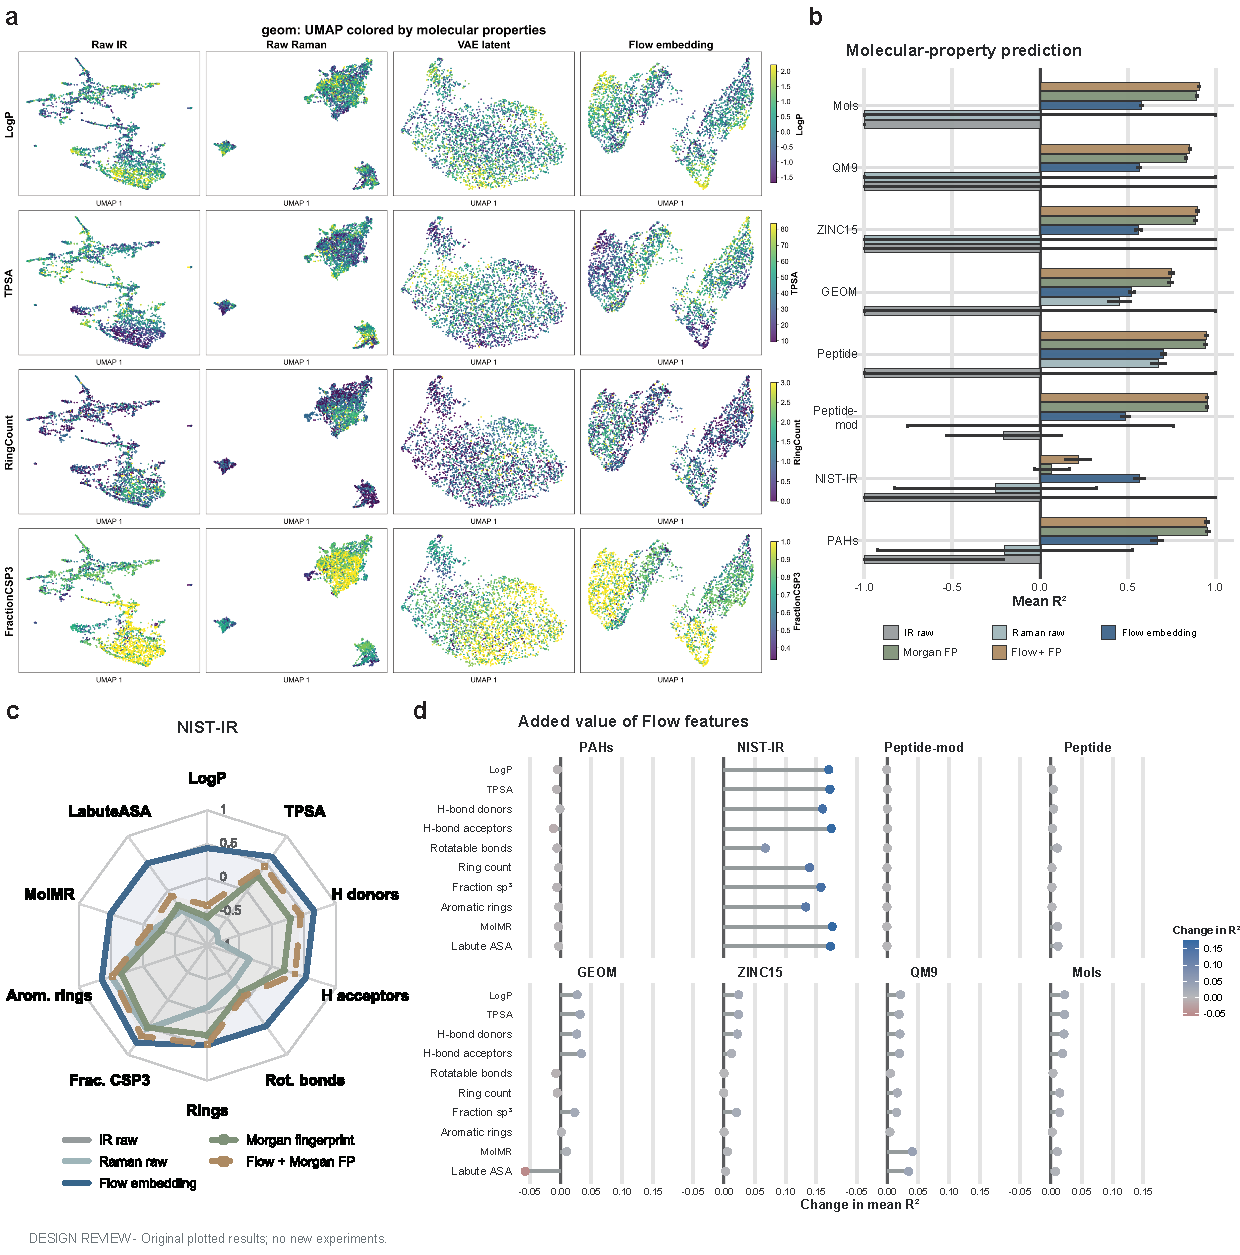
\includegraphics[width=\linewidth]{figs/results/result_3_draw_polished.pdf}
    \caption{\textbf{Molecular information in translation-trained spectral representations.}
\textbf{a,} GEOM UMAP projections of raw IR, raw Raman, VAE latent features and Flow embeddings, coloured by LogP, TPSA, ring count and fraction of sp$^3$ carbons. These projections illustrate representation structure; predictive performance is quantified by regression probes.
\textbf{b,} Mean downstream $R^2$ by dataset for ridge-regression probes using raw IR, raw Raman, Flow embeddings, Morgan fingerprints and concatenated Flow--fingerprint features.
\textbf{c,} Property-wise comparison on NIST-IR. The radar plot compares five feature sets across ten molecular descriptors.
\textbf{d,} Change in mean $R^2$ after adding Flow features to Morgan fingerprints. Positive and negative values indicate improved and reduced probe performance, respectively. Gains vary with property and dataset.}
    \label{fig:quantitative_result_3}
\end{figure}
